\section{Miniproject: The wheel}
\label{sec:the-wheel}
Before the main project's goal was defined, we studied and made experiments with the different sensors we had at hand, such as the hall sensor. We took a plastic wheel and attached small magnets on the wheel's spokes. Then, we made two small holes in the wheel's support and in each one we put a hall sensor. A small circuit with a panstamp was build to analyse the hall sensors' output signals. With the hall sensors signal pattern, we could determine the direction of movement and also the number of turns made in a period of time by the wheel. Figure~\ref{fig:wheel} shows the wheel along with the panstamp. 


\begin{figure}[h!]
 \centering
 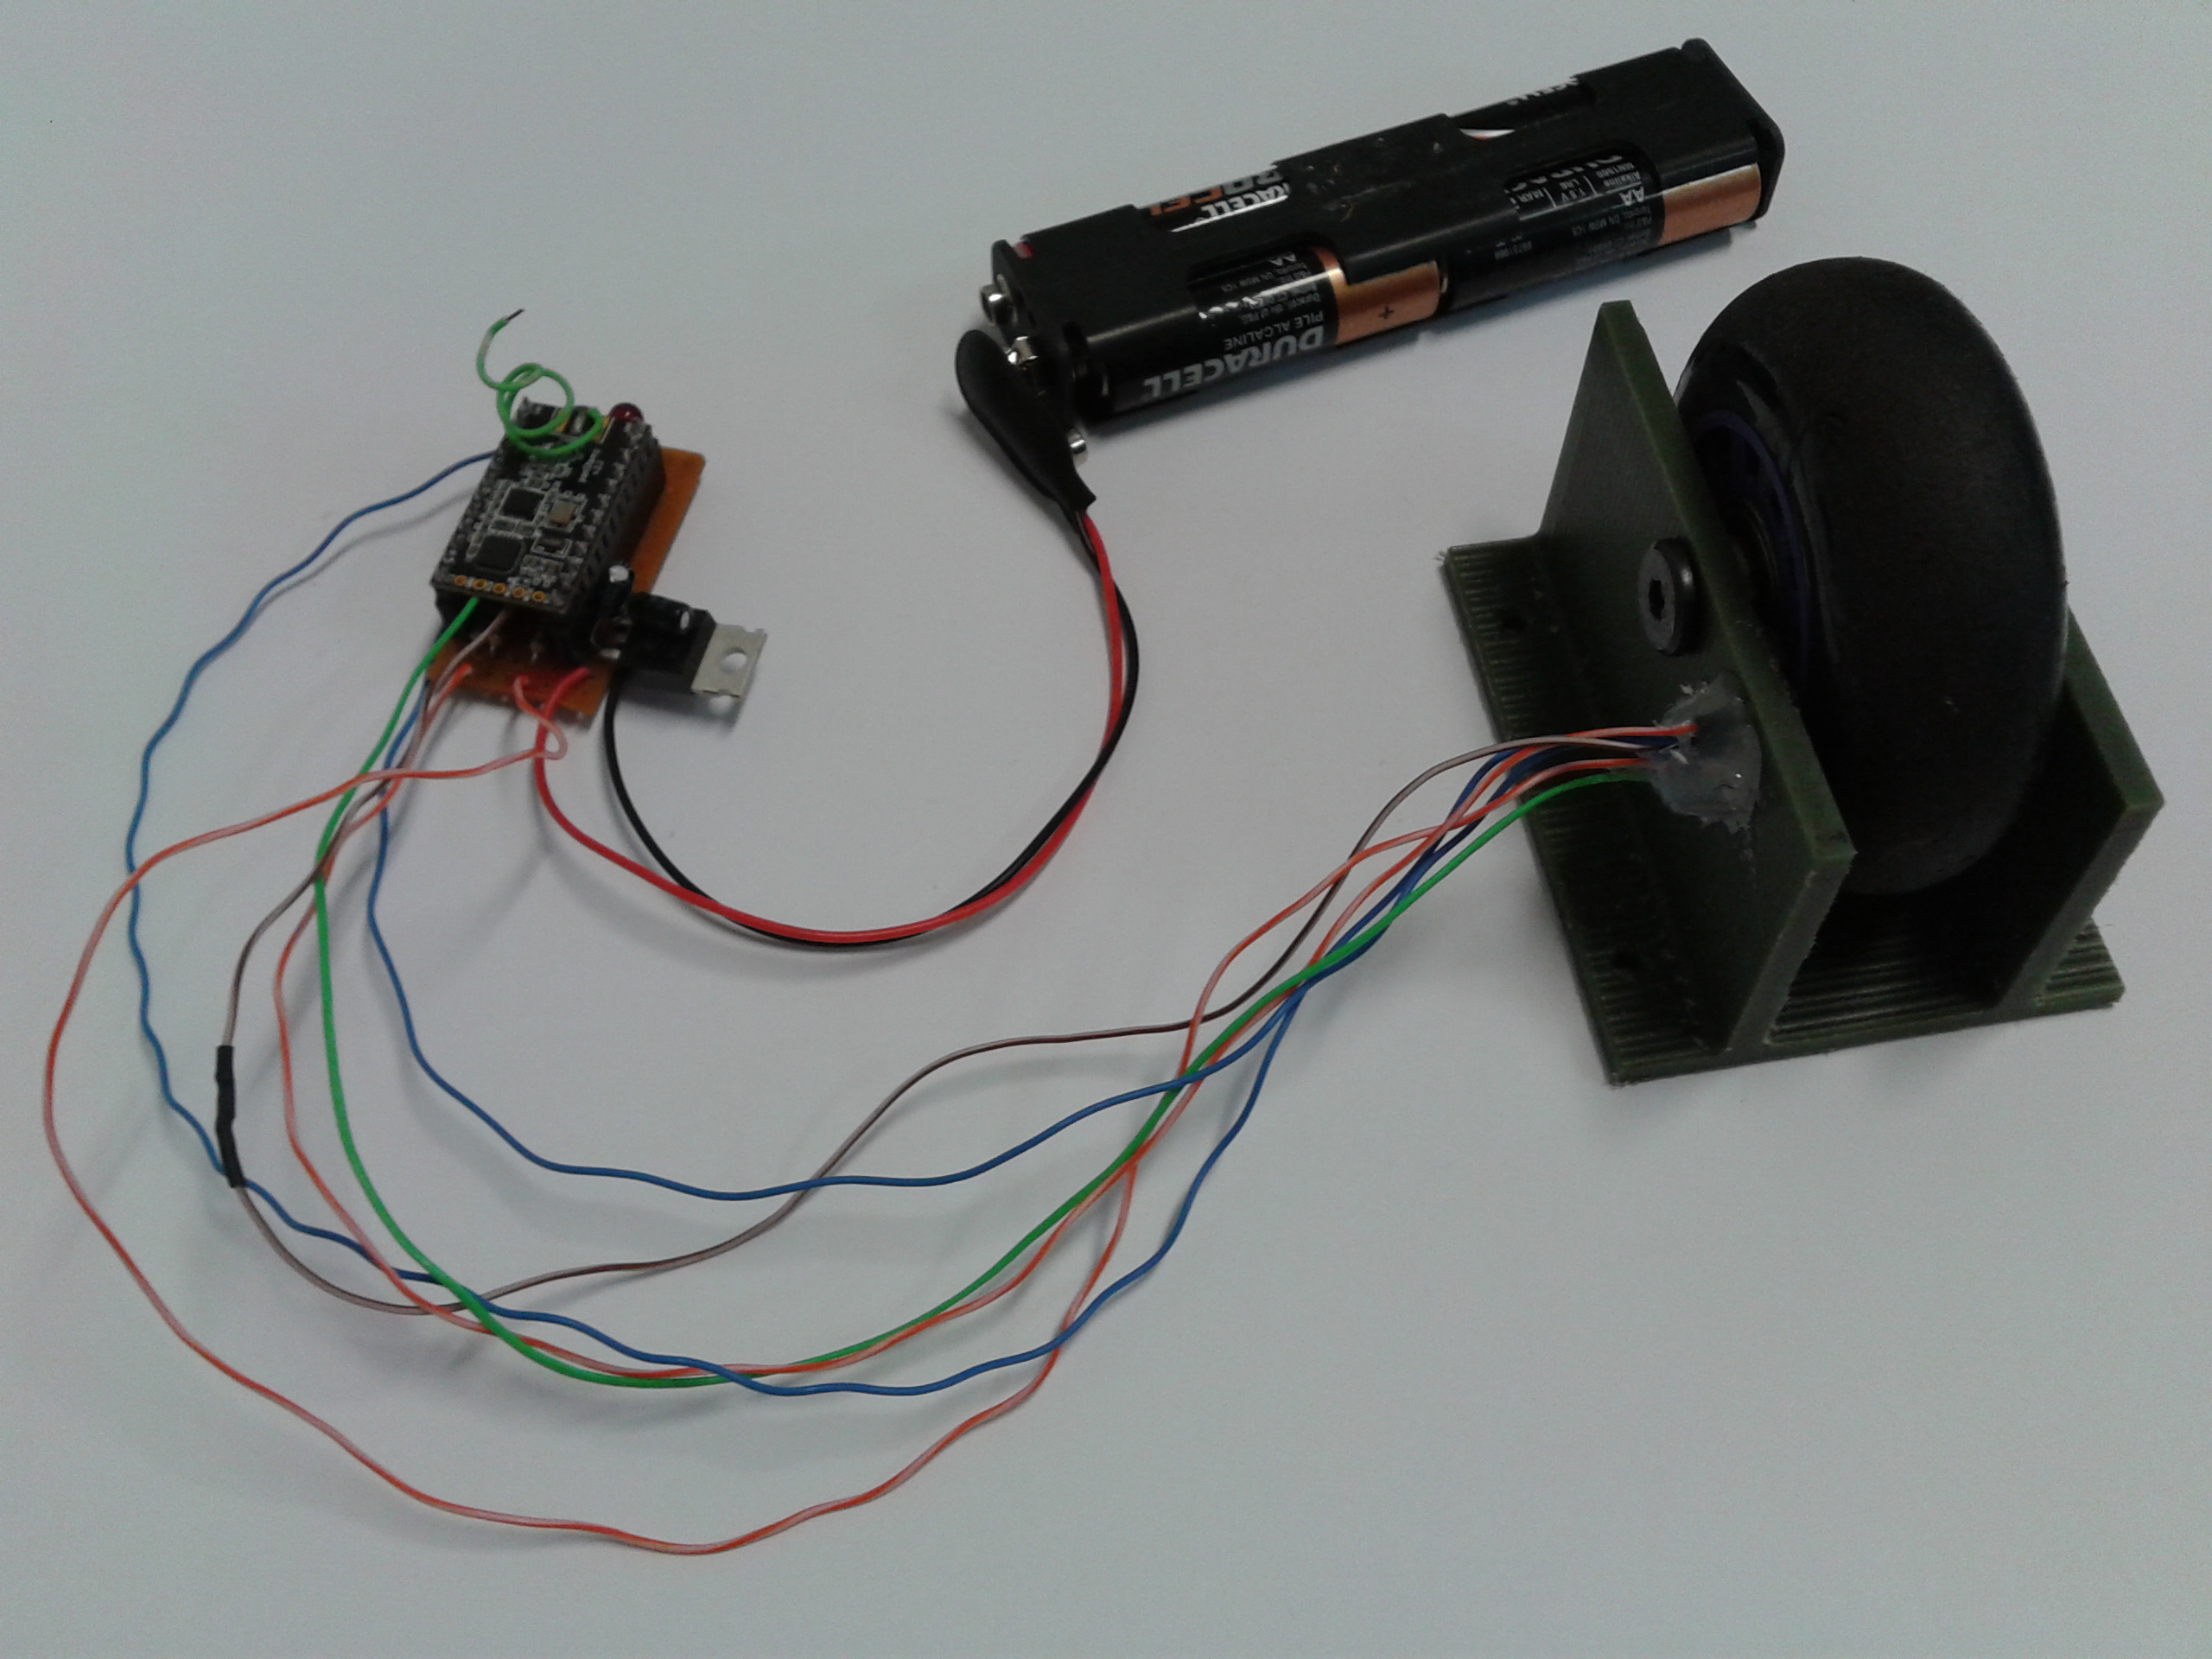
\includegraphics[width= 0.3\textwidth, clip=true  ,keepaspectratio=true]{./pic/wheel.jpg}
 \caption{The wheel and panstamp}
 \label{fig:wheel}
\end{figure}


\subsection{The hall sensor}
The sensor TLI4906 is a Hall Effect Switch, whose output depends on the magnetic field sensed by the chip (see  ). According to the datasheet, a magnetic south pole with a field strength above Bop (typical value 10 mTeslas) turns the output on, whereas a magnetic north pole exceeding Brp (typical value 8.5 mTeslas) turns it off. Figure~\ref{fig:hall-sensor-output}, taken from the datasheet, shows the relationship between the output voltage (named Vq) and the magnetic field sensed by the hall effect ship.

\begin{figure}[h!]
 \centering
 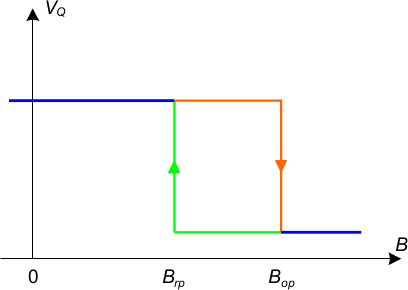
\includegraphics[width= 0.3\textwidth, clip=true  ,keepaspectratio=true]{./graph/hall-sensor-output.png}
 \caption{The hall sensor's output}
 \label{fig:hall-sensor-output}
\end{figure}

 After experimenting with the sensor, we realized that the absence of a magnet in front of the ship also turns the output off. With this property, we could distinguish two possible states:  magnet in front of the chip and no magnet in front of it. Since we were using to hall effect sensors, we could have 4 different states, as shown in Table~\ref{hall-sensor-output}. 
 
 
\begin{table}[h]
  \centering
  \begin{tabular}{ c | c | c | c}
    \hline
    \textbf{Sensor 1} & \textbf{Sensor 2} & \textbf{Vsensor1 } & \textbf{Vsensor2}\\ [0.5ex]    
    \hline
    No magnet & No magnet & 0 & 0 \\
    No magnet & Magnet & 0 & 1\\
    Magnet & No magnet & 1 & 0\\
    Magnet & Magnet & 1 & 1 \\      
    \hline
  \end{tabular}
  \caption[Output voltages in hall effect sensors]%
          {Possible output voltages combinations with the two hall effect sensors}
  \label{hall-sensor-output}
\end{table}

When the wheel rotates, the position of the magnets changes and this alters the combination of outputs of the hall effect sensors. The sequence of different states yields a pattern that can be used to determine the wheel's rotation direction (clockwise or counterclockwise)  In the next section, we describe how the hall effect output signals were processed by the panstamp.

\subsection{Processing the hall effect sensors' signals}

Figure~\ref{fig:Wheel-circuit} shows a simple diagram of the circuit built to determine the wheels direction of rotation. 

\begin{figure}[h!]
 \centering
 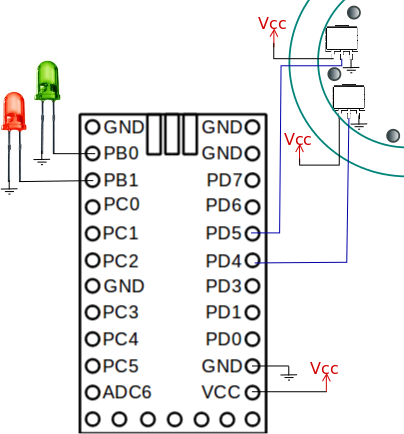
\includegraphics[width= 0.3\textwidth, clip=true  ,keepaspectratio=true]{./graph/wheel-circuit.png}
 \caption{Wheel circuit}
 \label{fig:Wheel-circuit}
\end{figure}

The output pin of each hall effect sensor was connected to a panstamp's digital output pin, namely PD4 and PD5.We configured an interruption, in the panstamp code, that is triggered with each change (rise and fall) in the voltage sensed by pin PD4. In interruption routine, the voltages in PD4 and PD5 were measured and a flag was raised. These voltage measurements were interpreted as binary inputs ('0' or '1') and constituted the trace that reflected the direction of rotation. The location of each magnet in the wheel's spokes was carefully selected to produce clear differences between the clockwise and the counterclockwise trace. The raised flag, mentioned before in the interruption routine, indicated if there was a change or not in the state; that is, if the wheel was rotating or not.

Without the library 'PinChangeInt.h', the only digital pins that can trigger this interruption are digital pins PD2 and PD3. Since the use of PD2 cannot be customized in the Panstamp, we had available just PD3. At the beginning, we thought we needed two interruptions (one triggered by PD4 and another by PD5) but Later, we realized that one interruption sufficed to do the analysis. 
In other words, we could have used pins PD3 and PD4 and configured interruptions with PD3 without the help of the above mentioned library. 

As explained in the arduino official website \cite{arduino}, it is useful to steer a digital input pin to a known state if no input is present. Writing a HIGH value with digitalWrite() in a digital pin, if if the pin is configured as an INPUT, will enable an internal 20K pullup resistor (to Vcc). On the other hand, writing LOW will disable the pullup. In our implementation, adding the internal pullup was fundamental to obtain the right readings of the hall effect sensor's output signals. 

Each time the panstamp detected movement in the wheel, it built a packet and sent it wirelessly to another panstamp that lit up a led strand. Two different packets were sent according to the direction of rotation and the leds in the led strand were lit in a way that reflected the two different directions. For debugging purposes, a led was lit when a certain direction of rotation was detected: the green led indicated clockwise rotation whereas the red one counter-clockwise rotation. 

This mini-project is a simple example of how the hall effect sensors, along with a panstamp, can be used to produce interactive systems. 








